% Foliensatz: "AFu-Kurs nach DJ4UF" von DK0TU, Amateurfunkgruppe der TU Berlin
% Lizenz: CC BY-NC-SA 3.0 de (http://creativecommons.org/licenses/by-nc-sa/3.0/de/)
% Autoren: Martin Deutschmann

\documentclass[aspectratio=169]{beamer}

\usepackage[ngerman]{babel} % deutsche Worttrennung etc.
\usepackage[utf8]{inputenc} % UTF8 Text

\usepackage[super, comma, numbers, square, sort]{natbib}

\usepackage{hyperref}       % Hyperref Package für bessere Referenzen (todo)
\hypersetup{
	colorlinks=false,       %   false: boxed links; true: colored links
    %linkcolor=white,       %   color of internal links (change box color with linkbordercolor)
    citecolor=red,          %   color of links to bibliography
    filecolor=white,        %   color of file links
    urlcolor=blue           %   color of external links
}

\usepackage{multirow}
\usepackage{wasysym}  % Math Symbols like \permil
%\usepackage{colortbl}
%\usepackage{subscript}
%\usepackage{caption}
%\usepackage{setspace}
%\usepackage{xcolor}        % benutze CodeListe

% Footnote
%\usepackage{hanging}
%
%\setbeamertemplate{footnote}{%
%  \hangpara{2em}{1}%
%  \makebox[2em][l]{\insertfootnotemark}\footnotesize\insertfootnotetext\par%
%}


%\usepackage{pgf}
%\usepackage{tikz}
%\usetikzlibrary{arrows,automata}
%\usetikzlibrary{positioning}
%
%\tikzset{
%    state/.style={
%           rectangle,
%           rounded corners,
%           draw=black, very thick,
%           minimum height=2em,
%           minimum width=2pt,
%           inner sep=2pt,
%           text centered,
%           },
%}

%\usepackage{listings}
%\lstset{basicstyle=\small, numberstyle=\tiny, extendedchars=true, numbers=left, numbersep=5pt}
%\lstset{showtabs=false, showspaces=false, showstringspaces=false}
%%\lstset{backgroundcolor=\color{white!75!lightgray}, , frame=single}
%%\lstset{backgroundcolor=\color{white}}
%%\lstset{backgroundcolor=none}
%\lstset{keywordstyle=\color{blue!50!gray},  identifierstyle=\color{black}}
%\lstset{commentstyle=\color{green!50!gray}, stringstyle=\color{red!50!gray}}
%\lstset{language=C, fontadjust=true, tabsize=2, breaklines=true}
%\lstset{backgroundcolor=\color{white!75!lightgray}, caption=\lstname, frame=single}
%\lstset{emphstyle=\color{black}\fbox}
%
%% Keine "Listing:"-Caption
%\captionsetup{labelformat=empty,labelsep=none}
%
%% für mathematische Umgebungen
%\usepackage{amsmath,amsfonts,amssymb}
%
%\lstdefinestyle{Bash}{
%language=Bash,
%frame=single,
%rulecolor=\color{black},
%backgroundcolor=\color{gray!50},
%keywordstyle=\color{black},
%identifierstyle=,
%commentstyle=\color{black},
%stringstyle=\color{magenta!65!white},
%showstringspaces=false,
%basicstyle=\footnotesize\ttfamily\color{black},
%numbers=none,
%breaklines=true,
%captionpos=b
%}

%\usepackage{listings}
%
%\lstdefinestyle{basic}{
%    captionpos=t,%
%    basicstyle=\footnotesize\ttfamily,%
%    numberstyle=\tiny,%
%    numbers=left,%
%    stepnumber=1,%
%    frame=single,%
%    showspaces=false,%
%    showstringspaces=false,%
%    showtabs=false,%
%    %
%    keywordstyle=\color{blue},%
%    identifierstyle=,%
%    commentstyle=\color{gray},%
%    stringstyle=\color{magenta}%
%}



% fließende Boxen haben keinen Abstand
%\fboxsep0mm

% inkludiere Creative Commons Helper
%%%%%%%%%%%%%%%%%%%%%%%%%%%%%%%%%%%%%%%%%%%%%%%%%%%%%%%%%%%%%%%%
%% ccBeamer 0.1, 2007-07-02                                   %%
%% Written by Sebastian Pipping <webmaster@hartwork.org>      %%
%% ---------------------------------------------------------- %%
%% Licensed under Creative Commons Attribution-ShareAlike 3.0 %%
%% http://creativecommons.org/licenses/by-sa/3.0/             %%
%%%%%%%%%%%%%%%%%%%%%%%%%%%%%%%%%%%%%%%%%%%%%%%%%%%%%%%%%%%%%%%%


%% Images
\newcommand{\CcImageBy}[1]{%
	
\includegraphics[scale=#1]{texdata/creative_commons/cc_by_30.pdf}%
}
\newcommand{\CcImageCc}[1]{%
	
\includegraphics[scale=#1]{texdata/creative_commons/cc_cc_30.pdf}%
}
\newcommand{\CcImageDevNations}[1]{%
	
\includegraphics[scale=#1]{texdata/creative_commons/cc_dev_nations_30.pdf}%
}
\newcommand{\CcImageNc}[1]{%
	
\includegraphics[scale=#1]{texdata/creative_commons/cc_nc_30.pdf}%
}
\newcommand{\CcImageNd}[1]{%
	
\includegraphics[scale=#1]{texdata/creative_commons/cc_nd_30.pdf}%
}
\newcommand{\CcImagePd}[1]{%
	
\includegraphics[scale=#1]{texdata/creative_commons/cc_pd_30.pdf}%
}
\newcommand{\CcImageSa}[1]{%
	
\includegraphics[scale=#1]{texdata/creative_commons/cc_sa_30.pdf}%
}
\newcommand{\CcImageSampling}[1]{%
	
\includegraphics[scale=#1]{texdata/creative_commons/cc_sampling_30.pdf}%
}
\newcommand{\CcImageSamplingPlus}[1]{%
	
\includegraphics[scale=#1]{texdata/creative_commons/cc_sampling_plus_30.pdf}%
}


%% Groups
\newcommand{\CcGroupBy}[2]{% zoom, gap
	\CcImageCc{#1}\hspace*{#2}\CcImageBy{#1}%
}
\newcommand{\CcGroupByNc}[2]{% zoom, gap
	\CcImageCc{#1}\hspace*{#2}\CcImageBy{#1}\hspace*{#2}\CcImageNc{#1}%
}
\newcommand{\CcGroupByNcNd}[2]{% zoom, gap
	\CcImageCc{#1}\hspace*{#2}\CcImageBy{#1}\hspace*{#2}\CcImageNc{#1}\hspace*{#2}\CcImageNd{#1}%
}
\newcommand{\CcGroupByNcSa}[2]{% zoom, gap
	\CcImageCc{#1}\hspace*{#2}\CcImageBy{#1}\hspace*{#2}\CcImageNc{#1}\hspace*{#2}\CcImageSa{#1}%
}
\newcommand{\CcGroupByNd}[2]{% zoom, gap
	\CcImageCc{#1}\hspace*{#2}\CcImageBy{#1}\hspace*{#2}\CcImageNd{#1}%
}
\newcommand{\CcGroupBySa}[2]{% zoom, gap
	\CcImageCc{#1}\hspace*{#2}\CcImageBy{#1}\hspace*{#2}\CcImageSa{#1}%
}
\newcommand{\CcGroupDevNations}[2]{% zoom, gap
	\CcImageCc{#1}\hspace*{#2}\CcImageDevNations{#1}%
}
\newcommand{\CcGroupNcSampling}[2]{% zoom, gap
	\CcImageCc{#1}\hspace*{#2}\CcImageNc{#1}\hspace*{#2}\CcImageSampling{#1}%
}
\newcommand{\CcGroupPd}[1]{% zoom
	\CcImagePd{#1}%
}
\newcommand{\CcGroupSampling}[1]{% zoom
	\CcImageSampling{#1}%
}
\newcommand{\CcGroupSamplingPlus}[1]{% zoom
	\CcImageSamplingPlus{#1}%
}


%% Text
\newcommand{\CcLongnameBy}{Attribution}
\newcommand{\CcLongnameByNc}{Attribution-NonCommercial}
\newcommand{\CcLongnameByNcNd}{Attribution-NoDerivs}
\newcommand{\CcLongnameByNcSa}{Attribution-NonCommercial-ShareAlike}
\newcommand{\CcLongnameByNd}{Attribution-NoDerivs}
\newcommand{\CcLongnameBySa}{Attribution-ShareAlike}

\newcommand{\CcNote}[1]{% longname
	This work is licensed under the \textit{Creative Commons #1 3.0 License}.%
}


% generelles Thema auswählen
\usetheme{Goettingen} %Berlin spart ohne Sidebar allerdings angenehm Platz
% AnnArbor | Antibes | Bergen | Berkeley | Berlin | Boadilla | boxes | CambridgeUS | Copenhagen | Darmstadt | default | Dresden | Frankfurt | Goettingen | Hannover | Ilmenau | JuanLesPins | Luebeck | Madrid | Malmoe | Marburg | Montpellier | PaloAlto | Pittsburgh | Rochester | Singapore | Szeged | Warsaw

% Farben wählen
\usecolortheme{beetle}
% beaver | beetle | crane | default | dolphin | dove | fly | lily | orchid | rose | seagull | seahorse | sidebartab | structure | whale | wolverine

% Setze alle Farben auf Grau und Weiß
%\definecolor{craneorange}{RGB}{64,64,64}
%\definecolor{craneblue}{RGB}{255,255,255}

% Schriftart wählen
\usefonttheme{default}
% default | professionalfonts | serif | structurebold | structureitalicserif | structuresmallcapsserif

% Innere Themen(Kopf-, Fuß-, Sidebar usw)
%\useinnertheme{default}
\useinnertheme{circles}
% default | inmargin | rectangles | rounded | circles

% Äußere Themen (Anordnung der inneren, grenzen der Folien etc.)
\useoutertheme{infolines}
% default | infolines | miniframes | shadow | sidebar | smoothbars | smoothtree | split | tree

% Deaktiviere Navigations-Symbole ({} -> leer)
\setbeamertemplate{navigation symbols}{}
%\setbeamertemplate{navigation symbols}{\large \ifnum \insertframenumber <10 0\fi\insertframenumber/\inserttotalframenumber\vspace*{0.2ex}}

% Zeige ein Hintergrundbild
\setbeamertemplate{background canvas}{
        \hspace*{-2.0cm}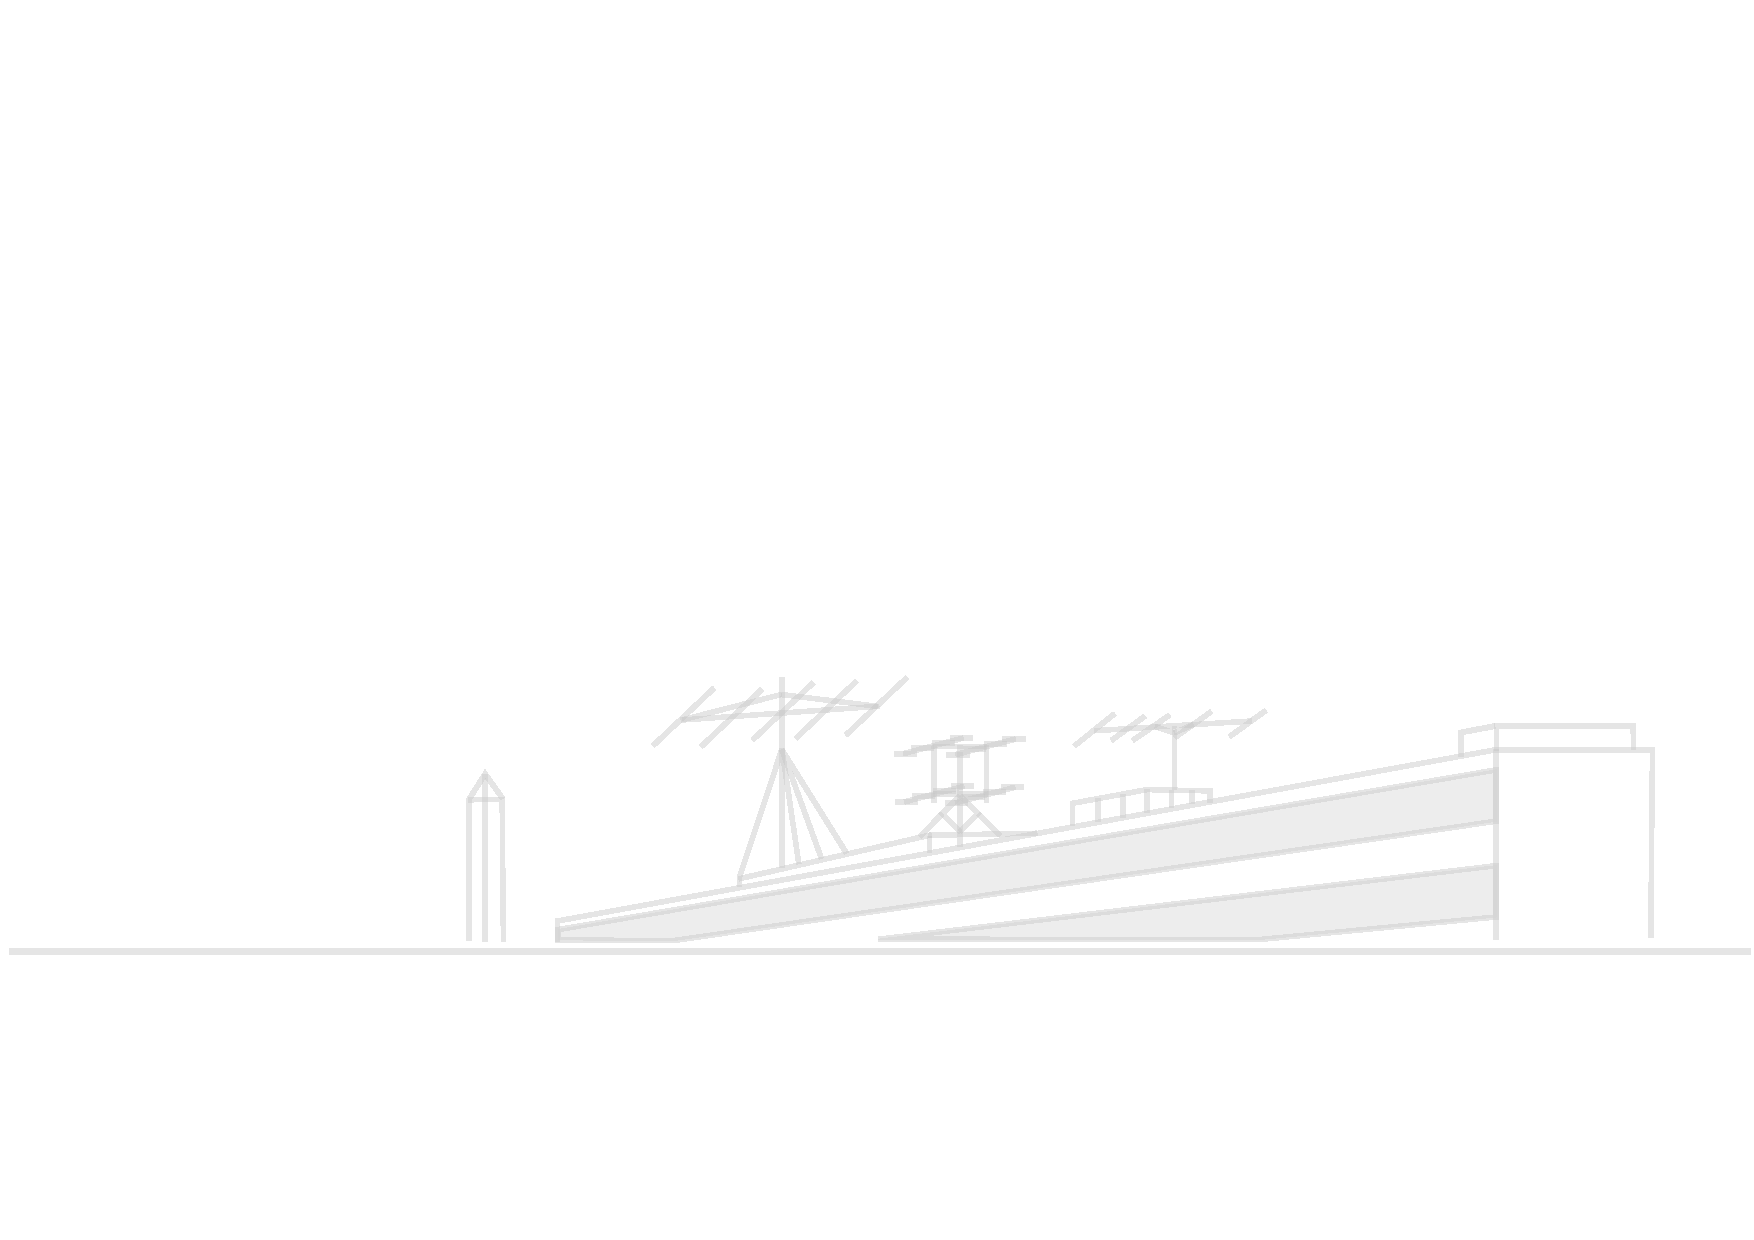
\includegraphics[width=17.8cm]{texdata/dk0tu_rooftop_background.pdf}
}

% Foliennummer einfügen
\setbeamertemplate{footline}[frame number]
%\setbeamertemplate{footline}{}

% Ändere das Zeichen vor jedem item
%\setbeamertemplate{itemize item}{\color{craneorange}$\blacktriangleright$}
%\setbeamertemplate{itemize subitem}{\color{craneorange}$\triangleright$}
%\setbeamertemplate{itemize subsubitem}{\color{craneorange}$\blacktriangleright$}

% Ändert die Blöcke 
\setbeamertemplate{blocks}[rounded][shadow=true]
% default | rounded [shadow=true|false]

%
% Eigene Kommandos
%

% Hack to get natbib and beamer working together. "The beamer user guide suggests
% that only the manual bibliography entry approach is supported"
% on some system it works out of the box, sometimes you need the hack :-(
% so check it --dl7bst
\ifdefined\newblock
    \relax
\else
    \newcommand{\newblock}{}
\fi

% \includedia command to generate png out of a dia file
% NEEDS installed dia and pdflatex option --shell-escape
\newcommand{\includedia}[1]{
    \immediate\write18{/usr/bin/dia #1.dia -e #1_diatmp.png -t png}
}

% RICHIG GROSSER FONT!
\newfont{\bigfont}{cmr10 at 144pt}
\newfont{\smallfont}{cmr10 at 8pt}

% Römische Ziffern
\makeatletter
\newcommand{\rmnum}[1]{\romannumeral #1}
\newcommand{\Rmnum}[1]{\expandafter\@slowromancap\romannumeral #1@}
\makeatother

% Schwarze Überschrift
%\setbeamercolor{frametitle}{fg=black}
%\setbeamercolor{title}{fg=black}

% Item- und Box-Farben
\definecolor{deepBlue}{HTML}{000066}
\setbeamercolor{itemize item}{fg=deepBlue}
\setbeamercolor{itemize subitem}{fg=deepBlue}
\setbeamercolor{description item}{fg=deepBlue}
\setbeamercolor{block title}{fg=deepBlue!100, bg=blue!15}
\setbeamercolor{block body}{fg=black, bg=blue!5}
\setbeamercolor{block title alerted}{fg=deepBlue, bg=red!75}
\setbeamercolor{block body alerted}{fg=black, bg=red!15}
\setbeamercolor*{block title example}{fg=blue!50, bg=blue!10}
\setbeamercolor*{block body example}{fg= blue, bg=blue!5}

%\setbeamercolor{section in head/foot}{parent=palette primary}
%\setbeamercolor{subsection in head/foot}{parent=palette secondary}
%\setbeamercolor{sidebar}{fg=darkblue,bg=yellow!90!orange}
%\setbeamercolor{title in sidebar}{fg=darkblue}
%\setbeamercolor{author in sidebar}{fg=darkblue}
%\setbeamercolor{section in sidebar}{fg=darkblue!10!black}
%\setbeamercolor{subsection in sidebar}{fg=darkblue!50!black}

% Titlepage Infos
\title{AFu-Kurs nach DJ4UF}
\author[DKØTU]{DKØTU\\ \footnotesize{Amateurfunkgruppe der TU Berlin}}
\institute[DKØTU]{\url{http://www.dk0tu.de} }

% PDF-Eigenschaften
\subject{DK0TU-Amateurfunkkurs nach DJ4UF}
\keywords{Amateurfunk Kurs HAM Radio Course CC-BY-NC-SA OpenSource TU Berlin DK0TU}

\subtitle{Technik Klasse E 14: \\
          Modulation \& Demodulation \\[2em]}
\date{Stand 08.01.2015}
 \begin{document}

\begin{frame}
    \titlepage
    \vfill
    \begin{center}
        \ccbyncsaeu\\
        {\tiny This work is licensed under the \em{Creative Commons Attribution-NonCommercial-ShareAlike 3.0 License}.}\\[0.5ex]
         \tiny Amateurfunkgruppe der Technische Universität Berlin (AfuTUB), DKØTU
         %\includegraphics[scale=0.5]{img/DK0TU_Logo.pdf}
    \end{center}
\end{frame}


%fixme Referenzen/Fußnoten-Systematik vereinheitlichen

\section*{Prinzip der Nachrichtenübertragung}
\begin{frame}
\frametitle{Prinzip der Nachrichtenübertragung}
\begin{center}
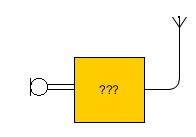
\includegraphics[scale=1.]{e14/Sender.png}\\
Abb. 1: Sender\\
\end{center}
\begin{itemize}
	\item Nachrichtentechnik in drahtgebundene und drahtlose eingeteilt
	\item Sender muss NF-Signal in HF-Signal umwandeln
	\item Dieser Vorgang wird Modulation genannt
	\item Demodulation macht aus einem HF-Signal ein NF-Signal
\end{itemize}
\end{frame}

\begin{frame}
\frametitle{Sendearten}
\begin{tiny}
\begin{minipage}{\textwidth}

\begin{minipage}{0.4\textwidth}
	\begin{tabular}{|l|l|}
	\hline
		\multicolumn{2}{|c|}{\textbf{1. Symbol: Modulation des Haupträgers}}\\
		\hline
		A & Zweiseitenband AM \\ \hline
		C & Restseitenband AM  \\ \hline
		F & Frequenzmodulation  \\ 
		G & Phasenmodulation\\ \hline
		J & Einseitenband AM, unterdrückter Träger\\ \hline		
	\end{tabular}
\end{minipage}
\hspace{1cm}
\begin{minipage}{0.4\textwidth}
	\begin{tabular}{|l|l|}
	\hline
		\multicolumn{2}{|c|}{\textbf{2. Symbol: Signalmodulation}}\\
		\hline
		" " & Einkanal mit quantisierter oder \\
		 1  & digitaler Information ohne \\
		" " & Modulation des Hilfsträgers \\ \hline		
		" " & Einkanal mit quantisierter oder\\
		 2  & digitaler Information mittels \\
		" " & eines modulierten Hilfsträgers \\ \hline	
		 3  & Einkanal mit analoger Modulation  \\ \hline	
	\end{tabular}
\end{minipage}
\end{minipage}
\vspace{0.5cm}
\begin{minipage}{0.4\textwidth}
	\begin{tabular}{|l|l|}
	\hline
		\multicolumn{2}{|c|}{\textbf{3. Symbol: Art der auszusendenden Information}}\\
		\hline
		A & Tastung durch Morsetelegrafie\\ \hline
		B & Fernschreiben \\ \hline
	    C & Faksimile(Bildübertragung)\\ \hline		
		D & Datenübertragung, Fernsteuerung\\ \hline
		E & Sprechfunk \\ \hline
		F & Fernsehen (Video)\\ \hline	
	\end{tabular}
\end{minipage}
\end{tiny}
\vspace{0.5cm}
\begin{itemize}
	\item Es gibt eine große Vielfalt von Sendearten
	\item zum Beispiel: J3E, A1A, F3E, C3F
\end{itemize}
\end{frame}

\begin{frame}
	\begin{small}	
	\begin{tabular}{|l|l|l|}
	\hline
		\multicolumn{3}{|c|}{\textbf{TD501: Durch Modulation...}}\\
		\hline
		A & werden Informationen auf einen & ??? \\
		" " &  oder mehrere Träger übertragen. & " " \\ \hline
		B & werden einem oder mehreren & ??? \\ 
		" " & Trägern Informationen entnommen.  & " " \\ \hline
		C & werden Sprach- und CW-Signale kombiniert.  & ??? \\ \hline
		D & werden dem Signal NF-Komponenten entnommen. & ??? \\ \hline 	
	\end{tabular}
	\end{small}
\end{frame}

\begin{frame}
	\begin{small}	
	\begin{tabular}{|l|l|l|}
	\hline
		\multicolumn{3}{|c|}{\textbf{TD501: Durch Modulation...}}\\
		\hline
		A & werden Informationen auf einen & Richtig \\
		" " &  oder mehrere Träger übertragen. & " " \\ \hline
		B & werden einem oder mehreren & ??? \\ 
		" " & Trägern Informationen entnommen.  & " " \\ \hline
		C & werden Sprach- und CW-Signale kombiniert.  & ??? \\ \hline
		D & werden dem Signal NF-Komponenten entnommen. & ??? \\ \hline 	
	\end{tabular}
	\end{small}
\end{frame}

\section*{Modulationsarten}
\begin{frame}
\frametitle{Modulationsarten}
\begin{center}
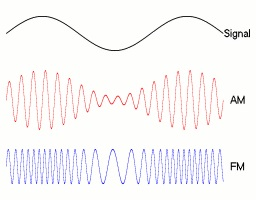
\includegraphics[scale=0.8]{e14/modulationen.jpg}\\
	Abb. 2: verschiedene Arten der Modulation
	\footnote{\url{http://upload.wikimedia.org/wikipedia/commons/a/a4/Amfm3-en-de.gif}}\\
	
\begin{itemize}
	\item grundsätzlich sind nur Amplitudenmodulation und Frequenzmodulation im Einsatz
	\item der eingefügte Träger muss sinusförmig sein
\end{itemize}
\end{center}
\end{frame}

\section{Amplitudenmodulation}
\begin{frame}
\frametitle{Amplitudenmodulation}
\begin{minipage}{0.4\textwidth}
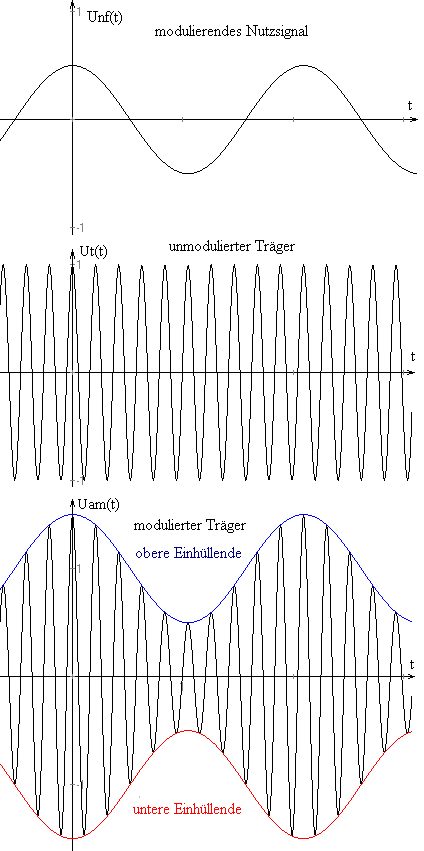
\includegraphics[scale=0.24]{e14/AM1.png}\\
\end{minipage}
\footnote{\url{http://upload.wikimedia.org/wikipedia/commons/b/b8/Amplitudenmodulation3.png}}
\hspace{0.5cm}
\begin{minipage}{0.4\textwidth}	
	\begin{itemize}
		\item wird nur noch im Rundfunk angewendet
		\item Information steckt in der Amplitude
		\item \url{http://upload.wikimedia.org/wikipedia/commons/6/62/Am2_spec.gif}
	\end{itemize}
\end{minipage}
\end{frame}

\section*{Modulationsgrad}
\begin{frame}
\frametitle{Modulationsgrad}
\begin{center}
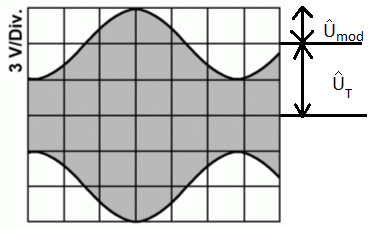
\includegraphics[scale=0.8]{e14/TE103.png}\\
Abb. 3: Modulationsgrade bei AM

\hspace{0.5cm}

\begin{itemize}
	\item	\LARGE{$m = \frac{\hat{U_{mod}}}{\hat{U_T}}$}
\end{itemize}
\end{center}
\end{frame}

\section*{Bandbreite bei AM}
\begin{frame}
\frametitle{Bandbreite bei AM}
\begin{center}
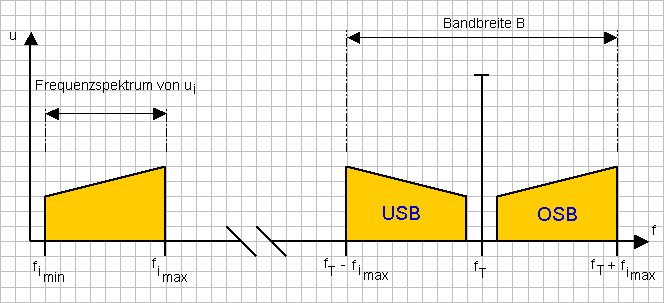
\includegraphics[scale=0.4]{e14/Bandbreite.png}\\
\footnote{\url{http://upload.wikimedia.org/wikipedia/commons/b/b9/Am_spek1.png}}
	\begin{itemize}
		\item Bandbreite ist die Differenz zwischen der höchsten und der niedrigsten Frequenz des HF-Signals
		\item Formel: \LARGE{$b_{AM} = 2 \cdot f_{NF,max}$}
	\end{itemize}
\end{center}
\end{frame}

\section*{Leistung bei AM}
\begin{frame}
\frametitle{Leistung bei AM}
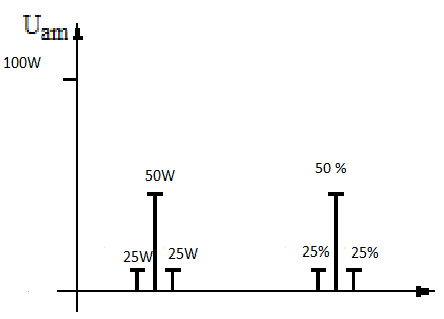
\includegraphics[scale=0.8]{e14/AMP.png}
\end{frame}

\section{Trägerunterdrückung (DSB)}
\begin{frame}
\frametitle{Trägerunterdrückung (DSB)}
\begin{itemize}
	\item Um Leistung zu sparen, kann der Träger unterdrückt werden
	\item Dies erfordert mehr Aufwand im Empfänger
	\item Nach dem umwandeln in ein HF-Signal wird der Träger herausgefiltert
	\item Die beiden Seitenbänder bleiben trotzdem als HF-Signal vorhanden
	\item Wird auch Doppelseitenbandmodulation genannt
	\item Im Amateurfunk nicht zulässig
\end{itemize}
\end{frame}

\section*{Einseitenbandmodulation SSB}
\begin{frame}
\frametitle{Einseitenbandmodulation SSB}
\begin{small}
\begin{itemize}
	\item \url{http://upload.wikimedia.org/wikipedia/commons/4/4e/Ssb_spec.gif}
	\item Um weitere Leistung zu sparen, kann man zusätzlich noch eines der Seitenbänder unterdrücken
	\item Dadurch wird die benötigte Bandbreite halbiert
	\item dies ist möglich, da beide Seitenbänder die gleiche Information beinhalten
	\item Im Amateurfunk wird unterhalb von 10 MHz das LSB und oberhalb von 10 MHz das USB genutzt	
	\item Die Bandbreite eines SSB-Signals ist identisch mit der Bandbreite des NF-Signals, also etwas geringer als die Hälfte der Bandbreite von AM.
	\item Bandbreite: $b_{SSB} = f_{NF,max} - f_{NF,min}$
	\item da $f_{NF,min}$ wesentlich kleiner als $f_{NF,max}$ gilt vereinfacht:
	\item $b_{SSB} = f_{NF,max}$
\end{itemize}
\end{small}
\end{frame}

\section*{Frequenzmodulation}
\begin{frame}
\frametitle{Frequenzmodulation}
	\begin{center}
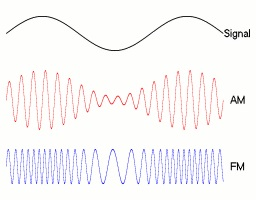
\includegraphics[scale=0.8]{e14/modulationen.jpg}\\
	Abb. 2: verschiedene Arten der Modulation
	\footnote{\url{http://upload.wikimedia.org/wikipedia/commons/a/a4/Amfm3-en-de.gif}}\\
	\begin{itemize}
		\item Wird im VHF / UHF Bereich angewandt
		\item Vor allem bei mobilem Funkbetrieb
		\item Findet auch bei Packet-Radio Anwendung
		\item Information steckt in der Frequenz
		\item Amplitude bleibt konstant
	\end{itemize}
	\end{center}
\end{frame}

\begin{frame}
\frametitle{Hub bei FM}
\begin{center}
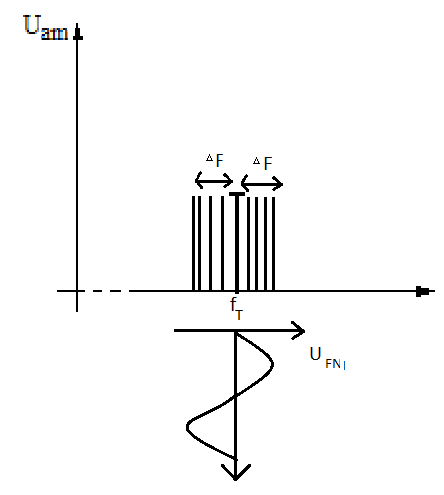
\includegraphics[scale=0.6]{e14/Hub.png}
\end{center}
\end{frame}

\section*{Bandbreite bei FM}
\begin{frame}
\frametitle{Bandbreite bei FM}
\begin{itemize}
	\item FM erzeugt Seitenbänder
	\item Im Amateurfunk wird ein geringer Hub verwendet, der die höchste vorkommende Niederfrequenz nicht überschreitet
	\item Dadurch gilt folgende Formel:
	\item \LARGE{$b_{FM} = 2 \cdot (\Delta f + f_{NF,max})$}
\end{itemize}
\end{frame}


\section*{FM pro \& contra}
\begin{frame}
\frametitle{FM Vor- \& Nachteile}
\textbf{\Large{Vorteile}}
\begin{itemize}
	\item Störungsicher, da die Amplitude konstant bleibt 
\end{itemize}
\vspace{1cm}
\textbf{\Large{Nachteile}}
\begin{itemize}
	\item benötigt mehr Bandbreite
	\item nur der stärkste Sender kann empfangen werden
\end{itemize}
\end{frame}


\section*{Referenzen}
\begin{frame}
    \frametitle{Referenzen/Links}
    
    \footnotesize
    \begin{itemize}
        \item Moltrecht E 14 : \\
              \url{http://www.darc.de/referate/ajw/ausbildung/darc-online-lehrgang/technik-klasse-e/technik-e14/}
		\item Fragenkatalog der BNetzA
			\url{http://www.dk0tu.de/Kurse/AFu-Lizenz/docs/TechnikFragenkatalogKlasseE.2006-09.pdf}
    \end{itemize}

\end{frame}

% Hier könnte noch eine Kontaktfolie stehen

\end{document}

